\documentclass[reqno, 11pt]{amsart}
\usepackage[dvipsnames]{xcolor}
\usepackage{tikz}
\usepackage{tikz-cd}
\usetikzlibrary{shapes,arrows,cd}
\usetikzlibrary{calc,arrows.meta,positioning}
\usetikzlibrary{decorations.pathreplacing}
\usepackage{mathrsfs,amssymb}
\usepackage{amsmath}
\usepackage[
breaklinks=true,colorlinks=true,
linkcolor=black,urlcolor=black,citecolor=black,% PRINT
bookmarks=true,bookmarksopenlevel=2]{hyperref}

\begin{document}

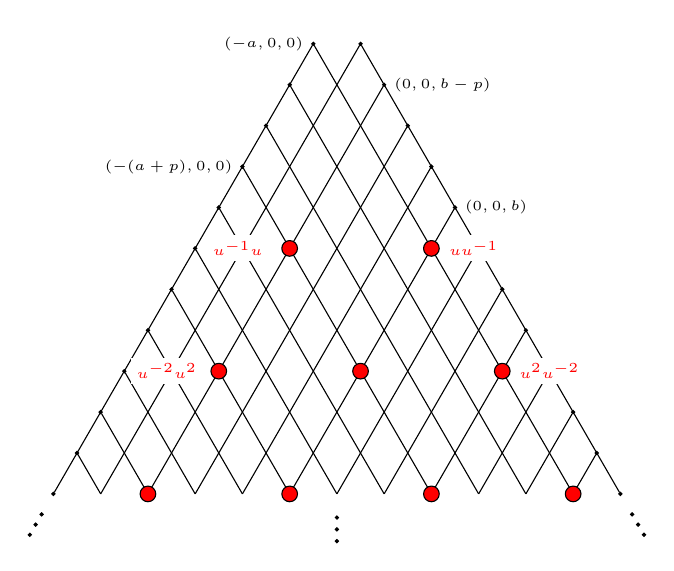
\begin{tikzpicture}[scale=0.6]
\node [draw, shape = circle, fill = black, inner sep=-2, scale=0.2] (f1) at (0.5,8) {};
\node[draw, shape=circle, fill=black, inner sep=-2, scale=0.2] (e1) at (-0.5,8) {}; 
\foreach \i in {2, ..., 12}{
    \node[draw, shape=circle, fill=black, inner sep=-2, scale=0.2] (f\i) at ($(f1)+(-60:\i-1)$) {};
    \node[draw, shape=circle, fill=black, inner sep=-2, scale=0.2] (e\i) at ($(e1)+(-120:\i-1)$) {};
}

\draw (f1)--(f12);
\draw (e1)--(e12);

\foreach \i in {1, ..., 11} {
    \draw (f\i) -- ($(e1)+(-120:11)+(0:\i)$);
    \draw (e\i) -- ($(f1)+(-60:11)-(0:\i)$);
}

\node[draw, shape = circle, fill=black, label=left:{\tiny $(-a,0,0)$}, inner sep=-1, scale=0.08] (ea) at (e1) {};
\node[draw, shape = circle, fill=black, label=left:{\tiny $(-(a+p),0,0)$}, inner sep=-1, scale=0.08] (eap) at (e4) {};
\node[draw, shape = circle, fill=black, label=right:{\tiny $(0,0,b-p)$}, inner sep=-1, scale=0.08] (fbp) at (f2) {};
\node[draw, shape = circle, fill=black, label=right:{\tiny $(0,0,b)$}, inner sep=-1, scale=0.08] (fb) at (f5) {};


\node [draw, shape = circle, fill = red, inner sep=-2] (m1) at ($(f6)-(0:1)$) {};
\node [red, fill=white,inner sep=2pt] at ($(m1)+(9mm,0mm)$) {\tiny $uu^{-1}$};

\node [draw, shape = circle, fill = red, inner sep=-2] (m'1) at ($(e6)+(0:2)$) {};
\node [red, fill=white, inner sep=2pt] at ($(m'1)+(-11mm,0mm)$) {\tiny $u^{-1}u$};

\node [draw, shape = circle, fill = red, inner sep=-2] (m2) at ($(f9)-(0:1)$) {};
\node [red, fill=white,inner sep=2pt] at ($(m2)+(10mm,0mm)$) {\tiny $u^2u^{-2}$};

\node [draw, shape = circle, fill = red, inner sep=-2] (m'2) at ($(e9)+(0:2)$) {};
\node [red, fill=white, inner sep=2pt] at ($(m'2)+(-11mm,0mm)$) {\tiny $u^{-2}u^2$};

\node [draw, shape = circle, fill = red, inner sep=-2] at ($(f9)-(0:4)$) {};



\node [draw, shape = circle, fill = red, inner sep=-2] at ($(f12)-(0:10)$) {};
\node [draw, shape = circle, fill = red, inner sep=-2] at ($(f12)-(0:7)$) {};
\node [draw, shape = circle, fill = red, inner sep=-2] at ($(f12)-(0:4)$) {};
\node [draw, shape = circle, fill = red, inner sep=-2] at ($(f12)-(0:1)$) {};
\node [draw, shape = circle, fill = black, inner sep=-2, scale=0.2] at ($(e12)+(-120:0.5)$) {};
\node [draw, shape = circle, fill = black, inner sep=-2, scale=0.2] at ($(e12)+(-120:0.75)$) {};
\node [draw, shape = circle, fill = black, inner sep=-2, scale=0.2] at ($(e12)+(-120:1)$) {};

\node [draw, shape = circle, fill = black, inner sep=-2, scale=0.2] at ($(e12)!0.5!(f12) + (-90:0.5)$) {};
\node [draw, shape = circle, fill = black, inner sep=-2, scale=0.2] at ($(e12)!0.5!(f12) + (-90:0.75)$) {};
\node [draw, shape = circle, fill = black, inner sep=-2, scale=0.2] at ($(e12)!0.5!(f12) + (-90:1)$) {};

\node [draw, shape = circle, fill = black, inner sep=-2, scale=0.2] at ($(f12)+(-60:0.5)$) {};
\node [draw, shape = circle, fill = black, inner sep=-2, scale=0.2] at ($(f12)+(-60:0.75)$) {};
\node [draw, shape = circle, fill = black, inner sep=-2, scale=0.2] at ($(f12)+(-60:1)$) {};

\end{tikzpicture}

\end{document}